\documentclass[11pt,a4paper]{article}

\usepackage[utf8]{inputenc}
\usepackage[T1]{fontenc}
% babel-turkish ile TikZ font komutları çakışıyor; sadece inputenc + T1
% kullanıp Türkçe karakterleri olduğu gibi gösteriyoruz.
\usepackage[a4paper,margin=2cm]{geometry}
\usepackage{tikz}
\usepackage{xcolor}
\usepackage{fancyhdr}
\usepackage{titlesec}
\usepackage{enumitem}
\usepackage{hyperref}
\usepackage{tabularx}
\usepackage{booktabs}

\usetikzlibrary{shapes.geometric, arrows.meta, positioning, calc}

\definecolor{accent}{HTML}{4f9cf9}
\definecolor{accent2}{HTML}{3ecf8e}
\definecolor{warn}{HTML}{f5a623}
\definecolor{danger}{HTML}{e74c3c}
\definecolor{purple}{HTML}{9b59b6}
\definecolor{slate}{HTML}{2a3447}
\definecolor{teal}{HTML}{1abc9c}

\tikzset{
  startStop/.style = {rectangle, rounded corners=10pt, draw=slate, very thick,
    fill=slate, text=white, minimum width=4cm, minimum height=0.85cm,
    align=center, font=\bfseries\small},
  process/.style = {rectangle, rounded corners=4pt, draw=accent, thick,
    fill=accent!12, minimum width=5cm, minimum height=0.85cm,
    align=center, font=\small},
  decision/.style = {diamond, aspect=2.5, draw=warn, thick, fill=warn!15,
    minimum width=4cm, align=center, font=\small, inner sep=2pt},
  approval/.style = {rectangle, rounded corners=4pt, draw=accent2, thick,
    fill=accent2!18, minimum width=5cm, minimum height=0.85cm,
    align=center, font=\small},
  reddet/.style = {rectangle, rounded corners=4pt, draw=danger, thick,
    fill=danger!12, minimum width=3.6cm, minimum height=0.75cm,
    align=center, font=\small},
  veri/.style = {rectangle, rounded corners=2pt, draw=purple, thick, dashed,
    fill=purple!10, minimum width=3.6cm, minimum height=0.75cm,
    align=center, font=\footnotesize},
  ok/.style = {-{Stealth[length=2.5mm]}, thick, draw=slate},
  okYes/.style = {-{Stealth[length=2.5mm]}, thick, draw=accent2},
  okNo/.style = {-{Stealth[length=2.5mm]}, thick, draw=danger},
  okDash/.style = {-{Stealth[length=2.5mm]}, thick, dashed, draw=purple},
}

\titleformat{\section}{\Large\bfseries\color{slate}}{\thesection}{0.5em}{}
\titleformat{\subsection}{\large\bfseries\color{accent}}{\thesubsection}{0.5em}{}

\pagestyle{fancy}
\fancyhf{}
\fancyhead[L]{\small\color{slate}\textbf{Arşen Process} -- Akış Şemaları}
\fancyhead[R]{\small\color{slate}\thepage}
\fancyfoot[C]{\small\color{slate}Fuwell · Syntegra}
\renewcommand{\headrulewidth}{0.4pt}

\hypersetup{
  colorlinks=true, linkcolor=accent, urlcolor=accent,
  pdftitle={Arşen Process -- Akış Şemaları},
  pdfauthor={Arşen Process Lab Takip Sistemi}
}

\begin{document}

\begin{titlepage}
\centering
\vspace*{3cm}
{\Huge\bfseries\color{slate} Arşen Process \par}
\vspace{0.4cm}
{\LARGE\color{accent} Lab ve Üretim Takip Sistemi \par}
\vspace{2cm}
{\Large\bfseries Akış Şemaları \par}
\vspace{0.3cm}
{\large\color{slate} Fuwell · Syntegra \par}
\vspace{3cm}
\begin{tabularx}{0.7\textwidth}{Xr}
\toprule
\textbf{Sürüm} & 1.0 \\
\textbf{Tarih} & \today \\
\textbf{Kapsam} & Sipariş + Proje + Onay Süreçleri \\
\bottomrule
\end{tabularx}
\vfill
{\small\color{slate}Şirket içi kullanım için hazırlanmıştır.}
\end{titlepage}

\tableofcontents
\newpage

% ============================================================================
\section{Giriş}

Bu doküman, \textbf{Arşen Process Lab ve Üretim Takip Sistemi} bünyesinde yer alan
iki ana iş akışını görsel olarak belgeler:

\begin{itemize}
  \item \textbf{Fuwell tarafı:} Müşteri siparişi alınması, üretim planlanması,
        süperkritik CO\textsubscript{2} ekstraksiyonu ile lot üretimi, analiz,
        formülasyon ve paketleme süreci.
  \item \textbf{Syntegra tarafı:} Proje açılması, mühendislik tasarımı, ekipman
        listesi oluşturulması, satın alma teklif yönetimi ve eşik kontrollü onay
        akışı.
\end{itemize}

Her iki süreçte de \textbf{Arşen Proses} şemsiyesi en üst kontrol kademesidir;
sorumlu atamaları yapar, kritik eşiklerde onay verir ve gerekli durumda her
kararı geri alabilir.

\vspace{0.6cm}
\noindent\textbf{Gösterim:}
\begin{tabularx}{\textwidth}{lX}
\textcolor{accent}{\rule{0.6cm}{0.25cm}} & Süreç adımı (kullanıcı eylemi) \\
\textcolor{accent2}{\rule{0.6cm}{0.25cm}} & Onay / başarılı çıkış \\
\textcolor{warn}{$\diamondsuit$} & Karar noktası \\
\textcolor{danger}{\rule{0.6cm}{0.25cm}} & Reddedilme / iptal \\
\textcolor{purple}{\rule{0.6cm}{0.25cm}} & Veri / referans kaydı \\
\textcolor{slate}{\rule{0.6cm}{0.25cm}} & Başlangıç / bitiş \\
\end{tabularx}

\newpage

% ============================================================================
% FUWELL
% ============================================================================
\section{Fuwell -- Sipariş ve Üretim Akışı}

Fuwell tarafı zeytinyağı üretim ve sipariş takibini yönetir. Akış, müşteri
siparişinden başlar ve son sevkiyata kadar her aşaması sistem üzerinde
belgelenir.

\subsection{Akış Şeması}

\begin{center}
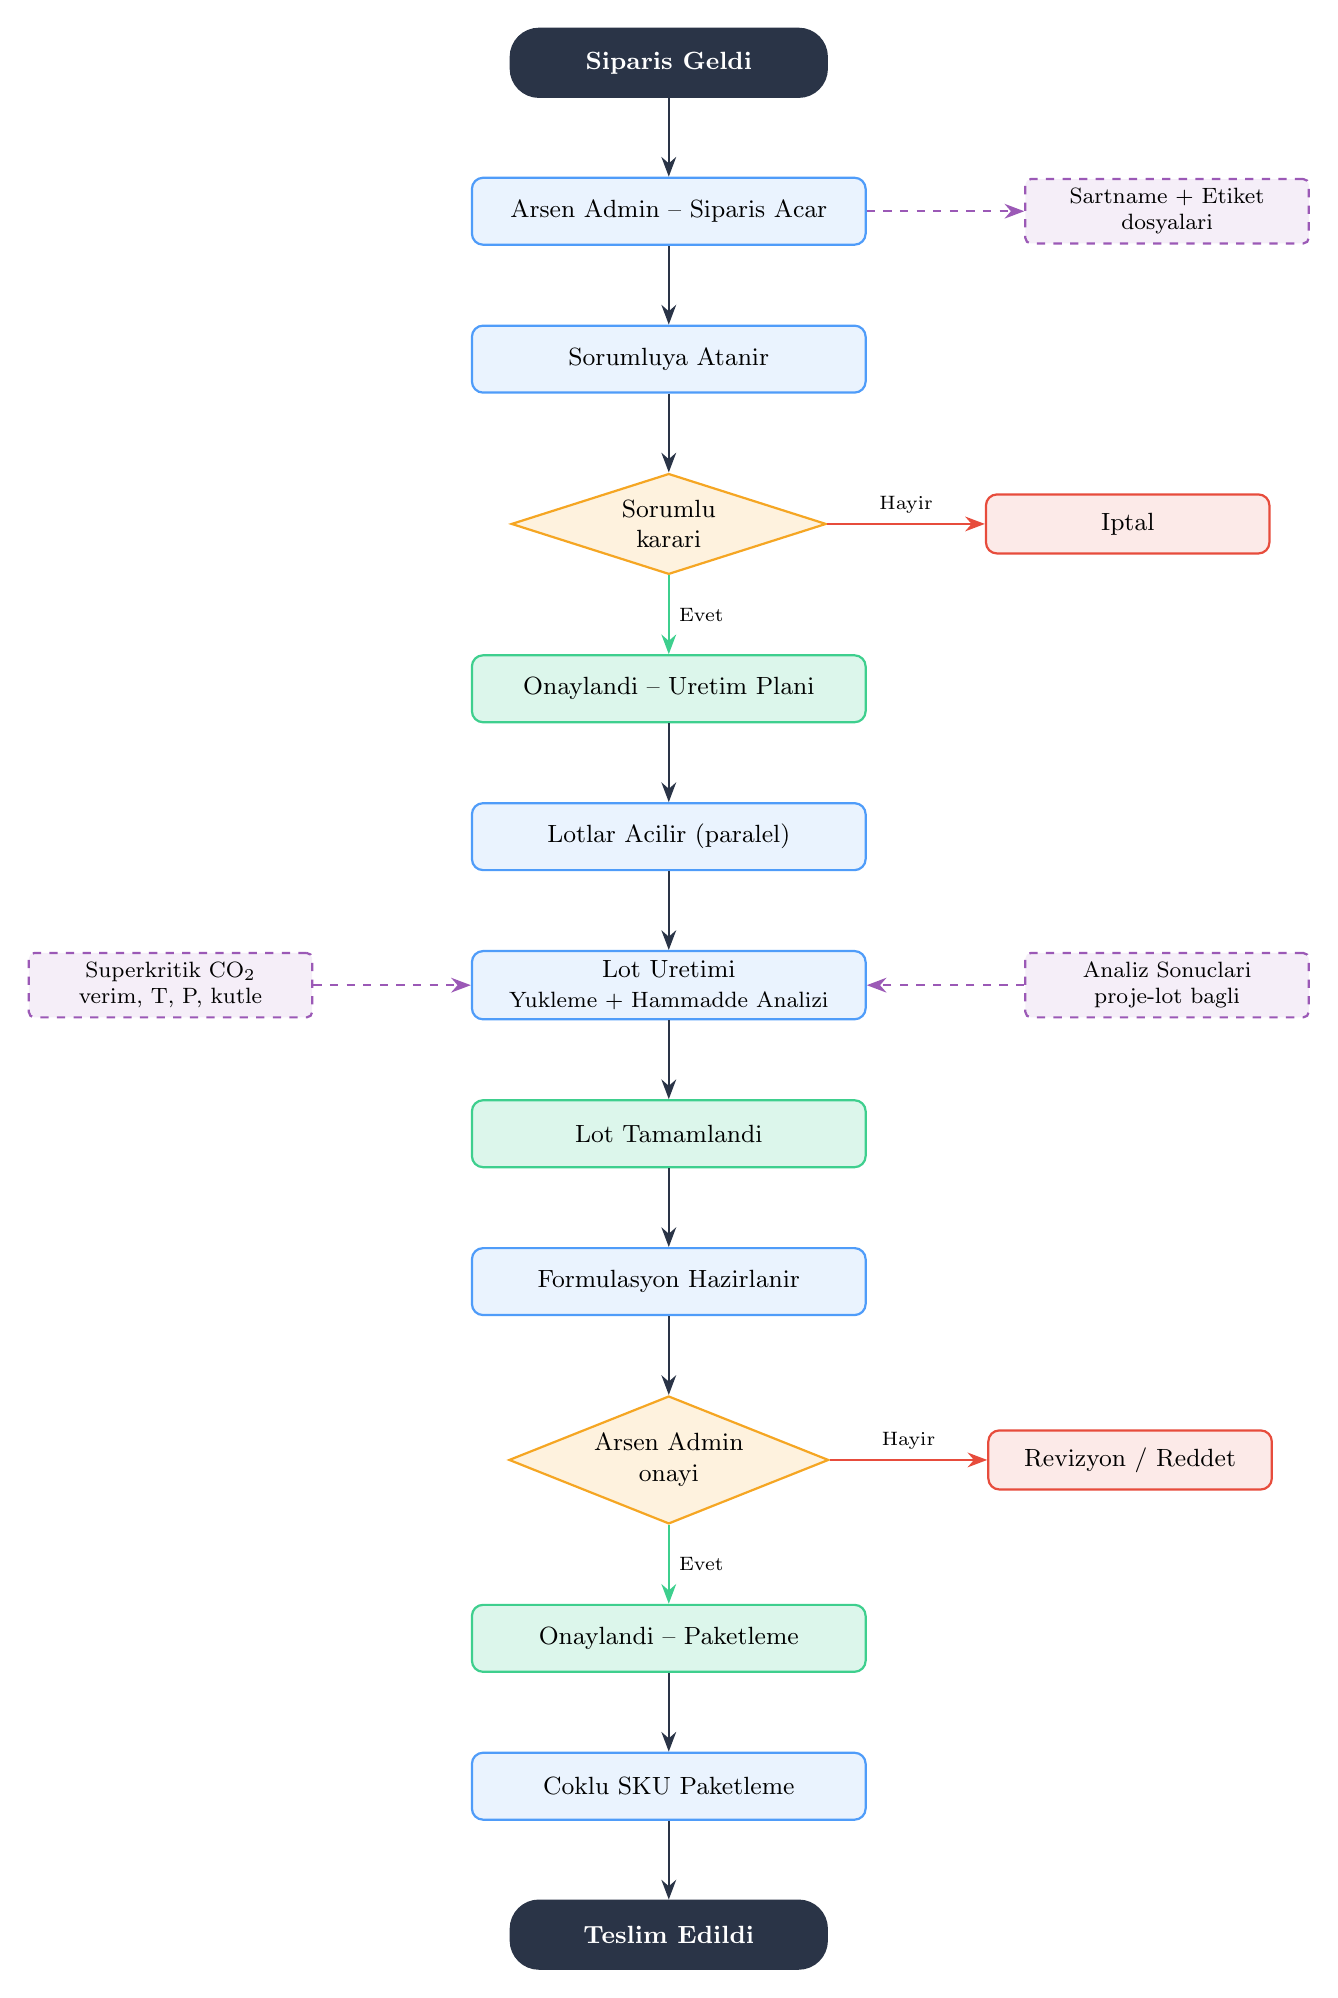
\begin{tikzpicture}[every node/.style={align=center}, node distance=1cm]

\node[startStop] (n1) {Siparis Geldi};
\node[process, below=of n1] (n2) {Arsen Admin -- Siparis Acar};
\node[veri, right=2cm of n2] (n2d) {Sartname + Etiket\\dosyalari};
\node[process, below=of n2] (n3) {Sorumluya Atanir};
\node[decision, below=of n3] (n4) {Sorumlu\\karari};
\node[reddet, right=2cm of n4] (n4r) {Iptal};
\node[approval, below=of n4] (n5) {Onaylandi -- Uretim Plani};
\node[process, below=of n5] (n6) {Lotlar Acilir (paralel)};
\node[process, below=of n6] (n7) {Lot Uretimi\\\footnotesize Yukleme + Hammadde Analizi};
\node[veri, left=2cm of n7] (n7d1) {Superkritik CO\textsubscript{2}\\verim, T, P, kutle};
\node[veri, right=2cm of n7] (n7d2) {Analiz Sonuclari\\proje-lot bagli};
\node[approval, below=of n7] (n8) {Lot Tamamlandi};
\node[process, below=of n8] (n9) {Formulasyon Hazirlanir};
\node[decision, below=of n9] (n10) {Arsen Admin\\onayi};
\node[reddet, right=2cm of n10] (n10r) {Revizyon / Reddet};
\node[approval, below=of n10] (n11) {Onaylandi -- Paketleme};
\node[process, below=of n11] (n12) {Coklu SKU Paketleme};
\node[startStop, below=of n12] (n13) {Teslim Edildi};

\draw[ok] (n1) -- (n2);
\draw[okDash] (n2) -- (n2d);
\draw[ok] (n2) -- (n3);
\draw[ok] (n3) -- (n4);
\draw[okNo] (n4) -- node[above, font=\scriptsize]{Hayir} (n4r);
\draw[okYes] (n4) -- node[right, font=\scriptsize]{Evet} (n5);
\draw[ok] (n5) -- (n6);
\draw[ok] (n6) -- (n7);
\draw[okDash] (n7d1) -- (n7);
\draw[okDash] (n7d2) -- (n7);
\draw[ok] (n7) -- (n8);
\draw[ok] (n8) -- (n9);
\draw[ok] (n9) -- (n10);
\draw[okNo] (n10) -- node[above, font=\scriptsize]{Hayir} (n10r);
\draw[okYes] (n10) -- node[right, font=\scriptsize]{Evet} (n11);
\draw[ok] (n11) -- (n12);
\draw[ok] (n12) -- (n13);

\end{tikzpicture}
\end{center}

\newpage

\subsection{Aşama Detayları}

\begin{tabularx}{\textwidth}{p{3.4cm}p{3cm}X}
\toprule
\textbf{Aşama} & \textbf{Yetkili} & \textbf{Yapılan İş} \\
\midrule
1. Sipariş Aç & Arşen Admin & Yeni siparişe FUW-YYYY-NNN-X kodu otomatik atanır; müşteri, ürün, hedef miktar, başlangıç ve termin girilir; şartname ve etiket dosyaları Drive klasörüne yüklenir. Sorumlu seçilir. \\
\addlinespace
2. Sorumluya Atama & Sistem $\rightarrow$ Sorumlu & Atanan sorumluya hem sistem içi bildirim hem e-posta gönderilir. \\
\addlinespace
3. Sorumlu Onayı & Atanan Sorumlu veya Admin & Sorumlu siparişi Onayla / Reddet eder. Onaylanmadan lot eklenemez. Reddetme sebebi zorunludur. Admin gerektiğinde kararı geri alabilir. \\
\addlinespace
4. Lot Açılışı (Paralel) & Sorumlu veya Admin & Bir sipariş için birden fazla lot paralel açılır. Her lot için lot no, planlanan miktar, sorumlu ve planlanan bitiş tarihi girilir. \\
\addlinespace
5. Yüklemeler & Operatör veya Mühendis & Her lota bir veya daha fazla süperkritik CO\textsubscript{2} yüklemesi eklenir: metot, sıcaklık, basınç, akış, süre, hammadde ve çıktı kütlesi, verim (otomatik hesaplanır). \\
\addlinespace
6. Analizler & Mühendis & Analiz Sonuçları sayfasından Proje-Lot alanı doldurulan analizler ilgili lota otomatik bağlanır. \\
\addlinespace
7. Formülasyon & Sorumlu & Tamamlanan lotlardan oranlar belirlenir; hedef ve gerçekleşen spek karşılaştırılır; Arşen onayına gönderilir. \\
\addlinespace
8. Arşen Onayı & Arşen Admin & Onayla / Reddet / Revizyon İste / Geri Al seçenekleri. Onaylanırsa sipariş Paketleme durumuna geçer. \\
\addlinespace
9. Paketleme & Operatör veya Admin & Çoklu SKU satırları: şişe tipi, hacim, adet, batch ID, sevkiyat termini, gönderim durumu. \\
\addlinespace
10. Teslimat & -- & Tüm SKU'lar Sevk Edildi olduğunda sipariş Teslim Edildi olarak işaretlenir. \\
\bottomrule
\end{tabularx}

\newpage

% ============================================================================
% SYNTEGRA
% ============================================================================
\section{Syntegra -- Proje ve Satın Alma Akışı}

Syntegra tarafı imalat projelerinin yönetimini içerir: mühendislik tasarımı,
ekipman listesi, satın alma teklif yönetimi ve eşik kontrollü Arşen onayı.

\subsection{Akış Şeması}

\begin{center}
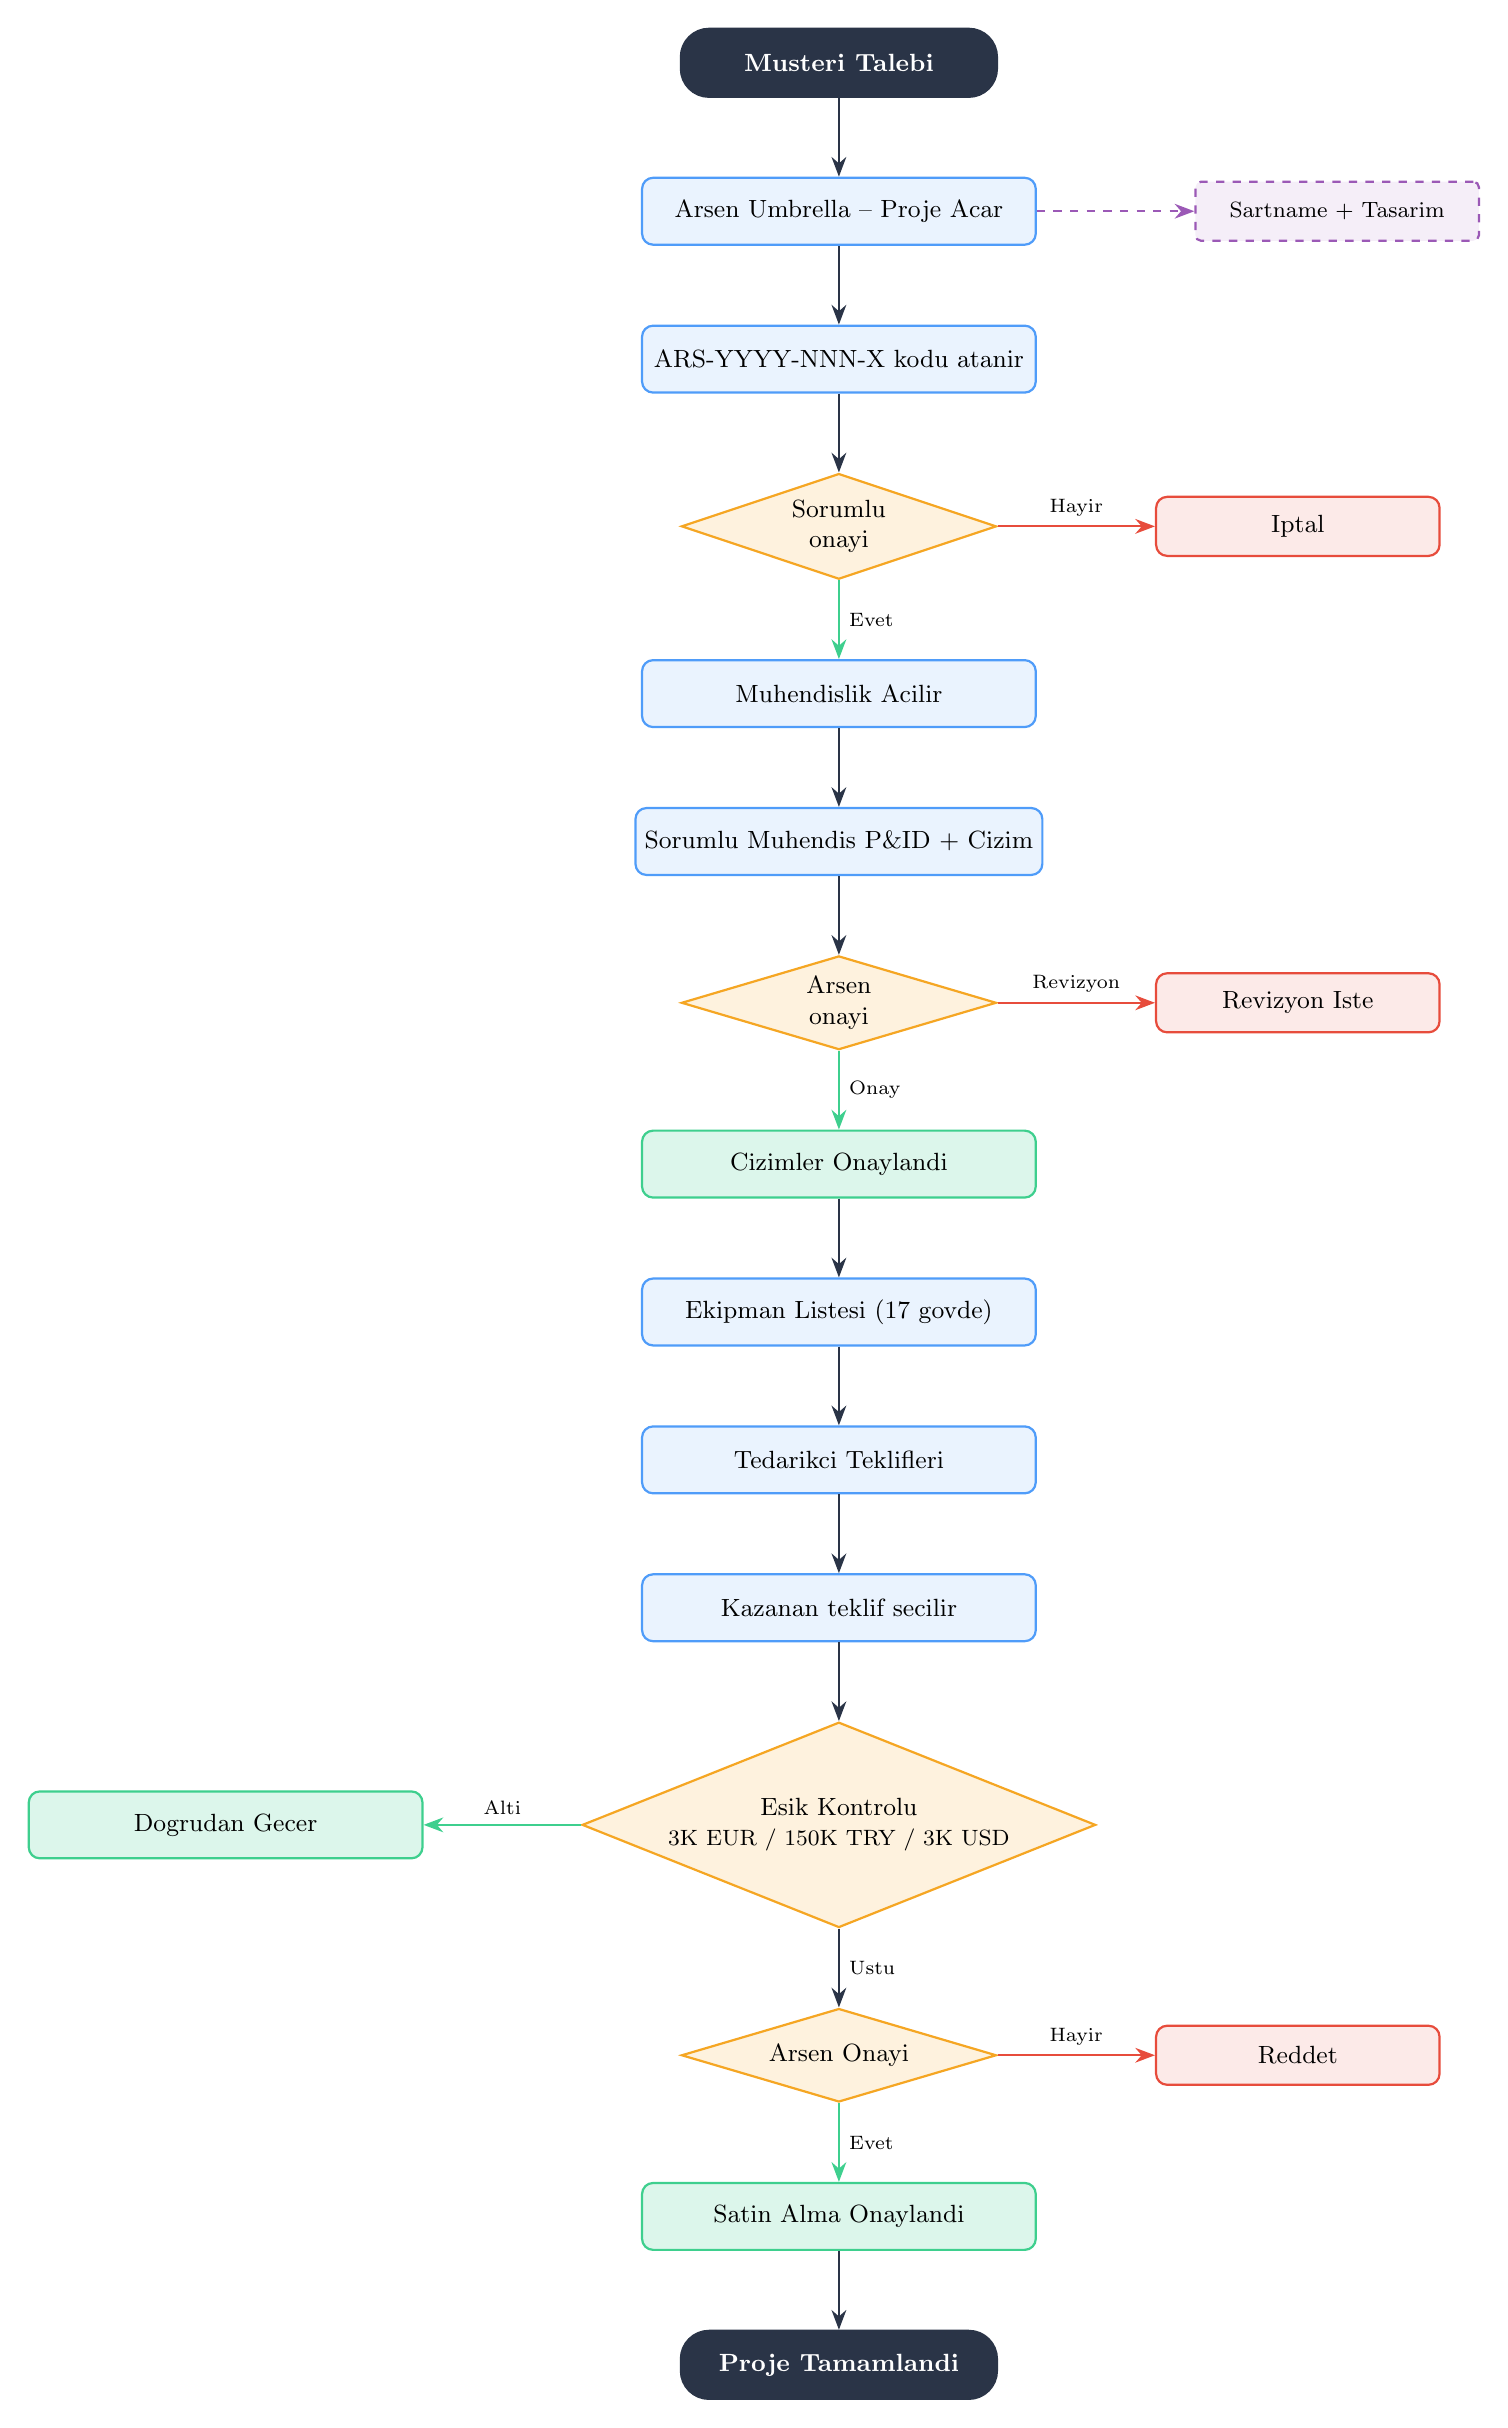
\begin{tikzpicture}[every node/.style={align=center}, node distance=1cm]

\node[startStop] (s1) {Musteri Talebi};
\node[process, below=of s1] (s2) {Arsen Umbrella -- Proje Acar};
\node[veri, right=2cm of s2] (s2d) {Sartname + Tasarim};
\node[process, below=of s2] (s3) {ARS-YYYY-NNN-X kodu atanir};
\node[decision, below=of s3] (s4) {Sorumlu\\onayi};
\node[reddet, right=2cm of s4] (s4r) {Iptal};
\node[process, below=of s4] (s5) {Muhendislik Acilir};
\node[process, below=of s5] (s6) {Sorumlu Muhendis P\&ID + Cizim};
\node[decision, below=of s6] (s7) {Arsen\\onayi};
\node[reddet, right=2cm of s7] (s7r) {Revizyon Iste};
\node[approval, below=of s7] (s8) {Cizimler Onaylandi};
\node[process, below=of s8] (s9) {Ekipman Listesi (17 govde)};
\node[process, below=of s9] (s10) {Tedarikci Teklifleri};
\node[process, below=of s10] (s11) {Kazanan teklif secilir};
\node[decision, below=of s11] (s12) {Esik Kontrolu\\\footnotesize 3K EUR / 150K TRY / 3K USD};
\node[approval, left=2cm of s12] (s12d) {Dogrudan Gecer};
\node[decision, below=of s12] (s13) {Arsen Onayi};
\node[reddet, right=2cm of s13] (s13r) {Reddet};
\node[approval, below=of s13] (s14) {Satin Alma Onaylandi};
\node[startStop, below=of s14] (s15) {Proje Tamamlandi};

\draw[ok] (s1) -- (s2);
\draw[okDash] (s2) -- (s2d);
\draw[ok] (s2) -- (s3);
\draw[ok] (s3) -- (s4);
\draw[okNo] (s4) -- node[above, font=\scriptsize]{Hayir} (s4r);
\draw[okYes] (s4) -- node[right, font=\scriptsize]{Evet} (s5);
\draw[ok] (s5) -- (s6);
\draw[ok] (s6) -- (s7);
\draw[okNo] (s7) -- node[above, font=\scriptsize]{Revizyon} (s7r);
\draw[okYes] (s7) -- node[right, font=\scriptsize]{Onay} (s8);
\draw[ok] (s8) -- (s9);
\draw[ok] (s9) -- (s10);
\draw[ok] (s10) -- (s11);
\draw[ok] (s11) -- (s12);
\draw[okYes] (s12) -- node[above, font=\scriptsize]{Alti} (s12d);
\draw[ok] (s12) -- node[right, font=\scriptsize]{Ustu} (s13);
\draw[okNo] (s13) -- node[above, font=\scriptsize]{Hayir} (s13r);
\draw[okYes] (s13) -- node[right, font=\scriptsize]{Evet} (s14);
\draw[ok] (s14) -- (s15);

\end{tikzpicture}
\end{center}

\newpage

\subsection{Aşama Detayları}

\begin{tabularx}{\textwidth}{p{3.4cm}p{3cm}X}
\toprule
\textbf{Aşama} & \textbf{Yetkili} & \textbf{Yapılan İş} \\
\midrule
1. Proje Aç & Arşen Umbrella & Yeni projeye ARS-YYYY-NNN-X kodu atanır; müşteri, ürün, sorumlu (Syntegra çalışanı) ve termin girilir; şartname ile tasarım dosyaları Drive klasörüne yüklenir. \\
\addlinespace
2. Sorumluya Atama & Sistem $\rightarrow$ Sorumlu & Atanan Syntegra sorumlusuna sistem içi bildirim ve e-posta. \\
\addlinespace
3. Sorumlu Onayı & Atanan Sorumlu veya Admin & Sorumlu projeyi Onayla / Reddet eder. Onaylanmadan Mühendislik sekmesi açılmaz. \\
\addlinespace
4. Mühendislik & Atanan Mühendis & P\&ID ve çizim dosyaları yüklenir; satın alma sorumlusu seçilir; Arşen Onayına Gönder tıklanır. \\
\addlinespace
5. Arşen Mühendislik Onayı & Arşen Umbrella & Onayla / Revizyon İste / Geri Al. Revizyon sayısı sınırsızdır; her tur revizyon geçmişine kaydedilir. \\
\addlinespace
6. Ekipman Listesi & Mühendislik Sorumlusu & 17 gövde kategorisi (Gaz Rezerv, Sıvı Rezerv, Ekstraktör, Seperatör vb.); her gövde için alt-parçalar, adet, ölçü, malzeme cinsi ve kalitesi, amaç girilir. \\
\addlinespace
7. Satın Almaya Gönder & Mühendislik Sorumlusu & Onaylanan ekipman listesi otomatik olarak Satın Alma sekmesinde görünür. \\
\addlinespace
8. Teklif Yönetimi & Satın Alma Sorumlusu & Her alt-parça için birden fazla tedarikçi teklifi: fiyat, para birimi, termin, ödeme şekli, teslimat şekli. \\
\addlinespace
9. Kazanan Seçimi & Satın Alma Sorumlusu & Bir teklif kazanan olarak işaretlenir; sebep zorunludur. \\
\addlinespace
10. Eşik Kontrolü & Sistem (otomatik) & Aynı projedeki aynı tedarikçinin veya aynı ürünün kümülatif tutarı eşiği aşıyorsa Arşen onayı gerekir. Eşikler: 3.000 EUR / 150.000 TRY / 3.000 USD. \\
\addlinespace
11. Arşen Satın Alma Onayı & Arşen Umbrella & Onayla / Reddet / Geri Al. Reddedilirse başka teklif seçilmelidir. \\
\addlinespace
12. Tamamlandı & -- & Tüm onaylar bittiğinde proje Tamamlandı olarak işaretlenir. \\
\bottomrule
\end{tabularx}

\newpage

% ============================================================================
% YETKİ MATRİSİ
% ============================================================================
\section{Yetki Matrisi}

Aşağıdaki tablo, her aksiyon için hangi rolün yetkili olduğunu özetler.
\textbf{Arşen Admin} (umbrella) her zaman tüm kararları alabilir ve geri
alabilir.

\subsection{Fuwell}

\begin{tabularx}{\textwidth}{Xccc}
\toprule
\textbf{Aksiyon} & \textbf{Arşen Admin} & \textbf{Fuwell Admin} & \textbf{Sorumlu / Operatör} \\
\midrule
Sipariş açma & evet & evet & -- \\
Sorumlu onayı & evet (override) & evet & evet (atanan) \\
Lot ekleme & evet & evet & evet (atanan sorumlu) \\
Yükleme ekleme & evet & evet & evet (operatör) \\
Analiz kaydı & evet & evet & evet (mühendis) \\
Formülasyon hazırlama & evet & evet & evet (sorumlu) \\
\textbf{Formülasyon onayı} & \textbf{evet (yalnız bu rol)} & -- & -- \\
Paketleme & evet & evet & evet (operatör) \\
Karar geri al & evet & -- & -- \\
\bottomrule
\end{tabularx}

\vspace{1cm}

\subsection{Syntegra}

\begin{tabularx}{\textwidth}{Xccc}
\toprule
\textbf{Aksiyon} & \textbf{Arşen Umbrella} & \textbf{Syntegra Admin} & \textbf{Sorumlu} \\
\midrule
Proje açma & evet (yalnız bu rol) & -- & -- \\
Sorumlu onayı & evet (override) & evet & evet (atanan) \\
Mühendislik tasarımı & evet & evet & evet (atanan mühendis) \\
\textbf{Mühendislik onayı} & \textbf{evet (yalnız bu rol)} & -- & -- \\
Ekipman listesi & evet & evet & evet (sorumlu mühendis) \\
Teklif girme & evet & evet & evet (satın alma sorumlusu) \\
Kazanan seçimi & evet & evet & evet (satın alma sorumlusu) \\
\textbf{Satın alma onayı (eşik üstü)} & \textbf{evet (yalnız bu rol)} & -- & -- \\
Karar geri al & evet & -- & -- \\
\bottomrule
\end{tabularx}

\newpage

% ============================================================================
% VERİ AKIŞI
% ============================================================================
\section{Sistem Veri Akışı}

\subsection{Üst Seviye Mimari}

\begin{center}
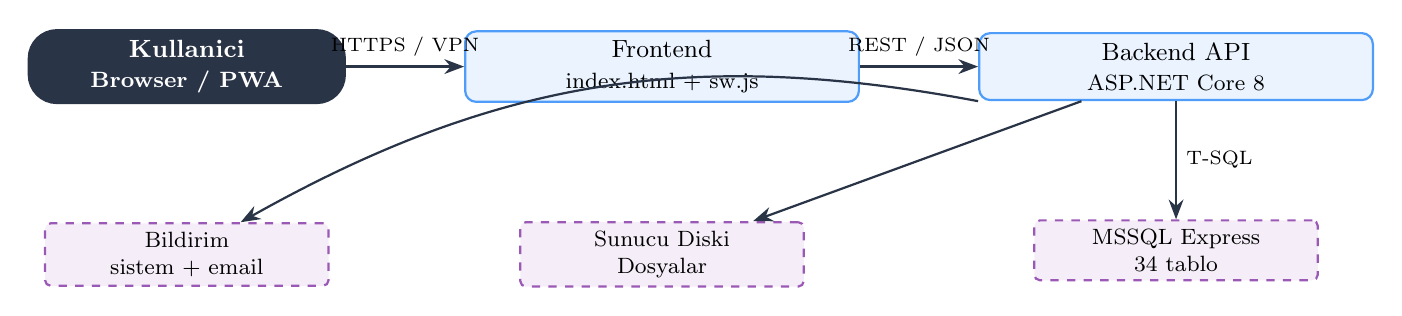
\begin{tikzpicture}[every node/.style={align=center}, node distance=1.5cm]
\node[startStop] (u) {Kullanici\\\footnotesize Browser / PWA};
\node[process, right=of u] (f) {Frontend\\\footnotesize index.html + sw.js};
\node[process, right=of f] (a) {Backend API\\\footnotesize ASP.NET Core 8};
\node[veri, below=of a] (db) {MSSQL Express\\34 tablo};
\node[veri, below=of f] (fs) {Sunucu Diski\\Dosyalar};
\node[veri, below=of u] (mail) {Bildirim\\\footnotesize sistem + email};

\draw[ok] (u) -- node[above, font=\scriptsize]{HTTPS / VPN} (f);
\draw[ok] (f) -- node[above, font=\scriptsize]{REST / JSON} (a);
\draw[ok] (a) -- node[right, font=\scriptsize]{T-SQL} (db);
\draw[ok] (a) -- (fs);
\draw[ok] (a.south west) to[bend right=20] (mail);
\end{tikzpicture}
\end{center}

\subsection{Entegrasyon Noktaları}

\begin{itemize}
  \item \textbf{Süperkritik CO\textsubscript{2} Hesaplayıcı:} Yapılan hesabı tek
        tıkla bir siparişe veya lota yükleme kaydı olarak işler (PR-EOS ile
        hesaplanan yoğunluk, sıkıştırılabilirlik dahil snapshot olarak
        saklanır).
  \item \textbf{Analiz Sonuçları:} Form üzerinde Proje-Lot alanı; doldurulursa
        analiz ilgili lotun alt-bilgisinde otomatik görünür.
  \item \textbf{Metodlar ve İzlekler:} Bir yükleme açılırken metot seçilir;
        metot sayfasında o metodun kaç yüklemede kullanıldığı sayılır.
  \item \textbf{Dosya Depolama:} Tek ortak klasör yapısı; her dosya için
        Fuwell, Syntegra veya Her İki Şirket görünürlük etiketi.
  \item \textbf{Bildirimler:} Atama ve karar değişikliklerinde otomatik (sistem
        içi bildirim + opsiyonel e-posta).
\end{itemize}

\newpage

% ============================================================================
% ÖZET
% ============================================================================
\section{Özet}

\begin{itemize}
  \item Her iki süreçte de \textbf{açık sorumluluk zinciri} vardır: hangi adımda
        kimin yetkili olduğu net şekilde belirlidir.
  \item \textbf{Arşen Proses} şemsiyesi her kararı override edebilir ve geri
        alabilir; böylece koordinasyon merkezi yetkide kalır.
  \item Tüm karar geçmişi (kim, ne zaman, hangi sebeple) \textbf{Onay Akışı /
        Geçmiş} kartında her projenin veya siparişin altında otomatik tutulur.
  \item Eşik kontrolleri (Syntegra satın alma), revizyon turları (Syntegra
        mühendislik) ve formülasyon onayı (Fuwell) için \textbf{otomatik akış
        yönlendirmesi} mevcuttur.
  \item Sistem, kullanıcıyı kara düzenden kurtarır: her görev atandığı kişiye
        bildirim olarak gider, takip eden kişi ekranda görür ve kararını verir.
\end{itemize}

\vspace{1cm}
\hrule
\vspace{0.4cm}
\noindent\small\textit{Bu doküman otomatik üretilmiştir. Süreç değişikliklerinde
güncellenmesi gereken yer: \texttt{server/docs/akis-semalari.tex}.}

\end{document}
